%!TEX root = ..\report.tex
\section{Results}
    \label{sec:results}
    \subsection{Network Architectures}
        The algorithm produces deep, interconnected architectures with ease. A variety of architectures is illustrated in \href{fig:arch}. Notice how the fully connected layer at the head of the network tends to dominate the total parameters for the model. This is to be expected with fully connected layers, however, this is a large source of latency in training.

        \begin{figure}[H]
            \centering
            \label{fig:arch}
            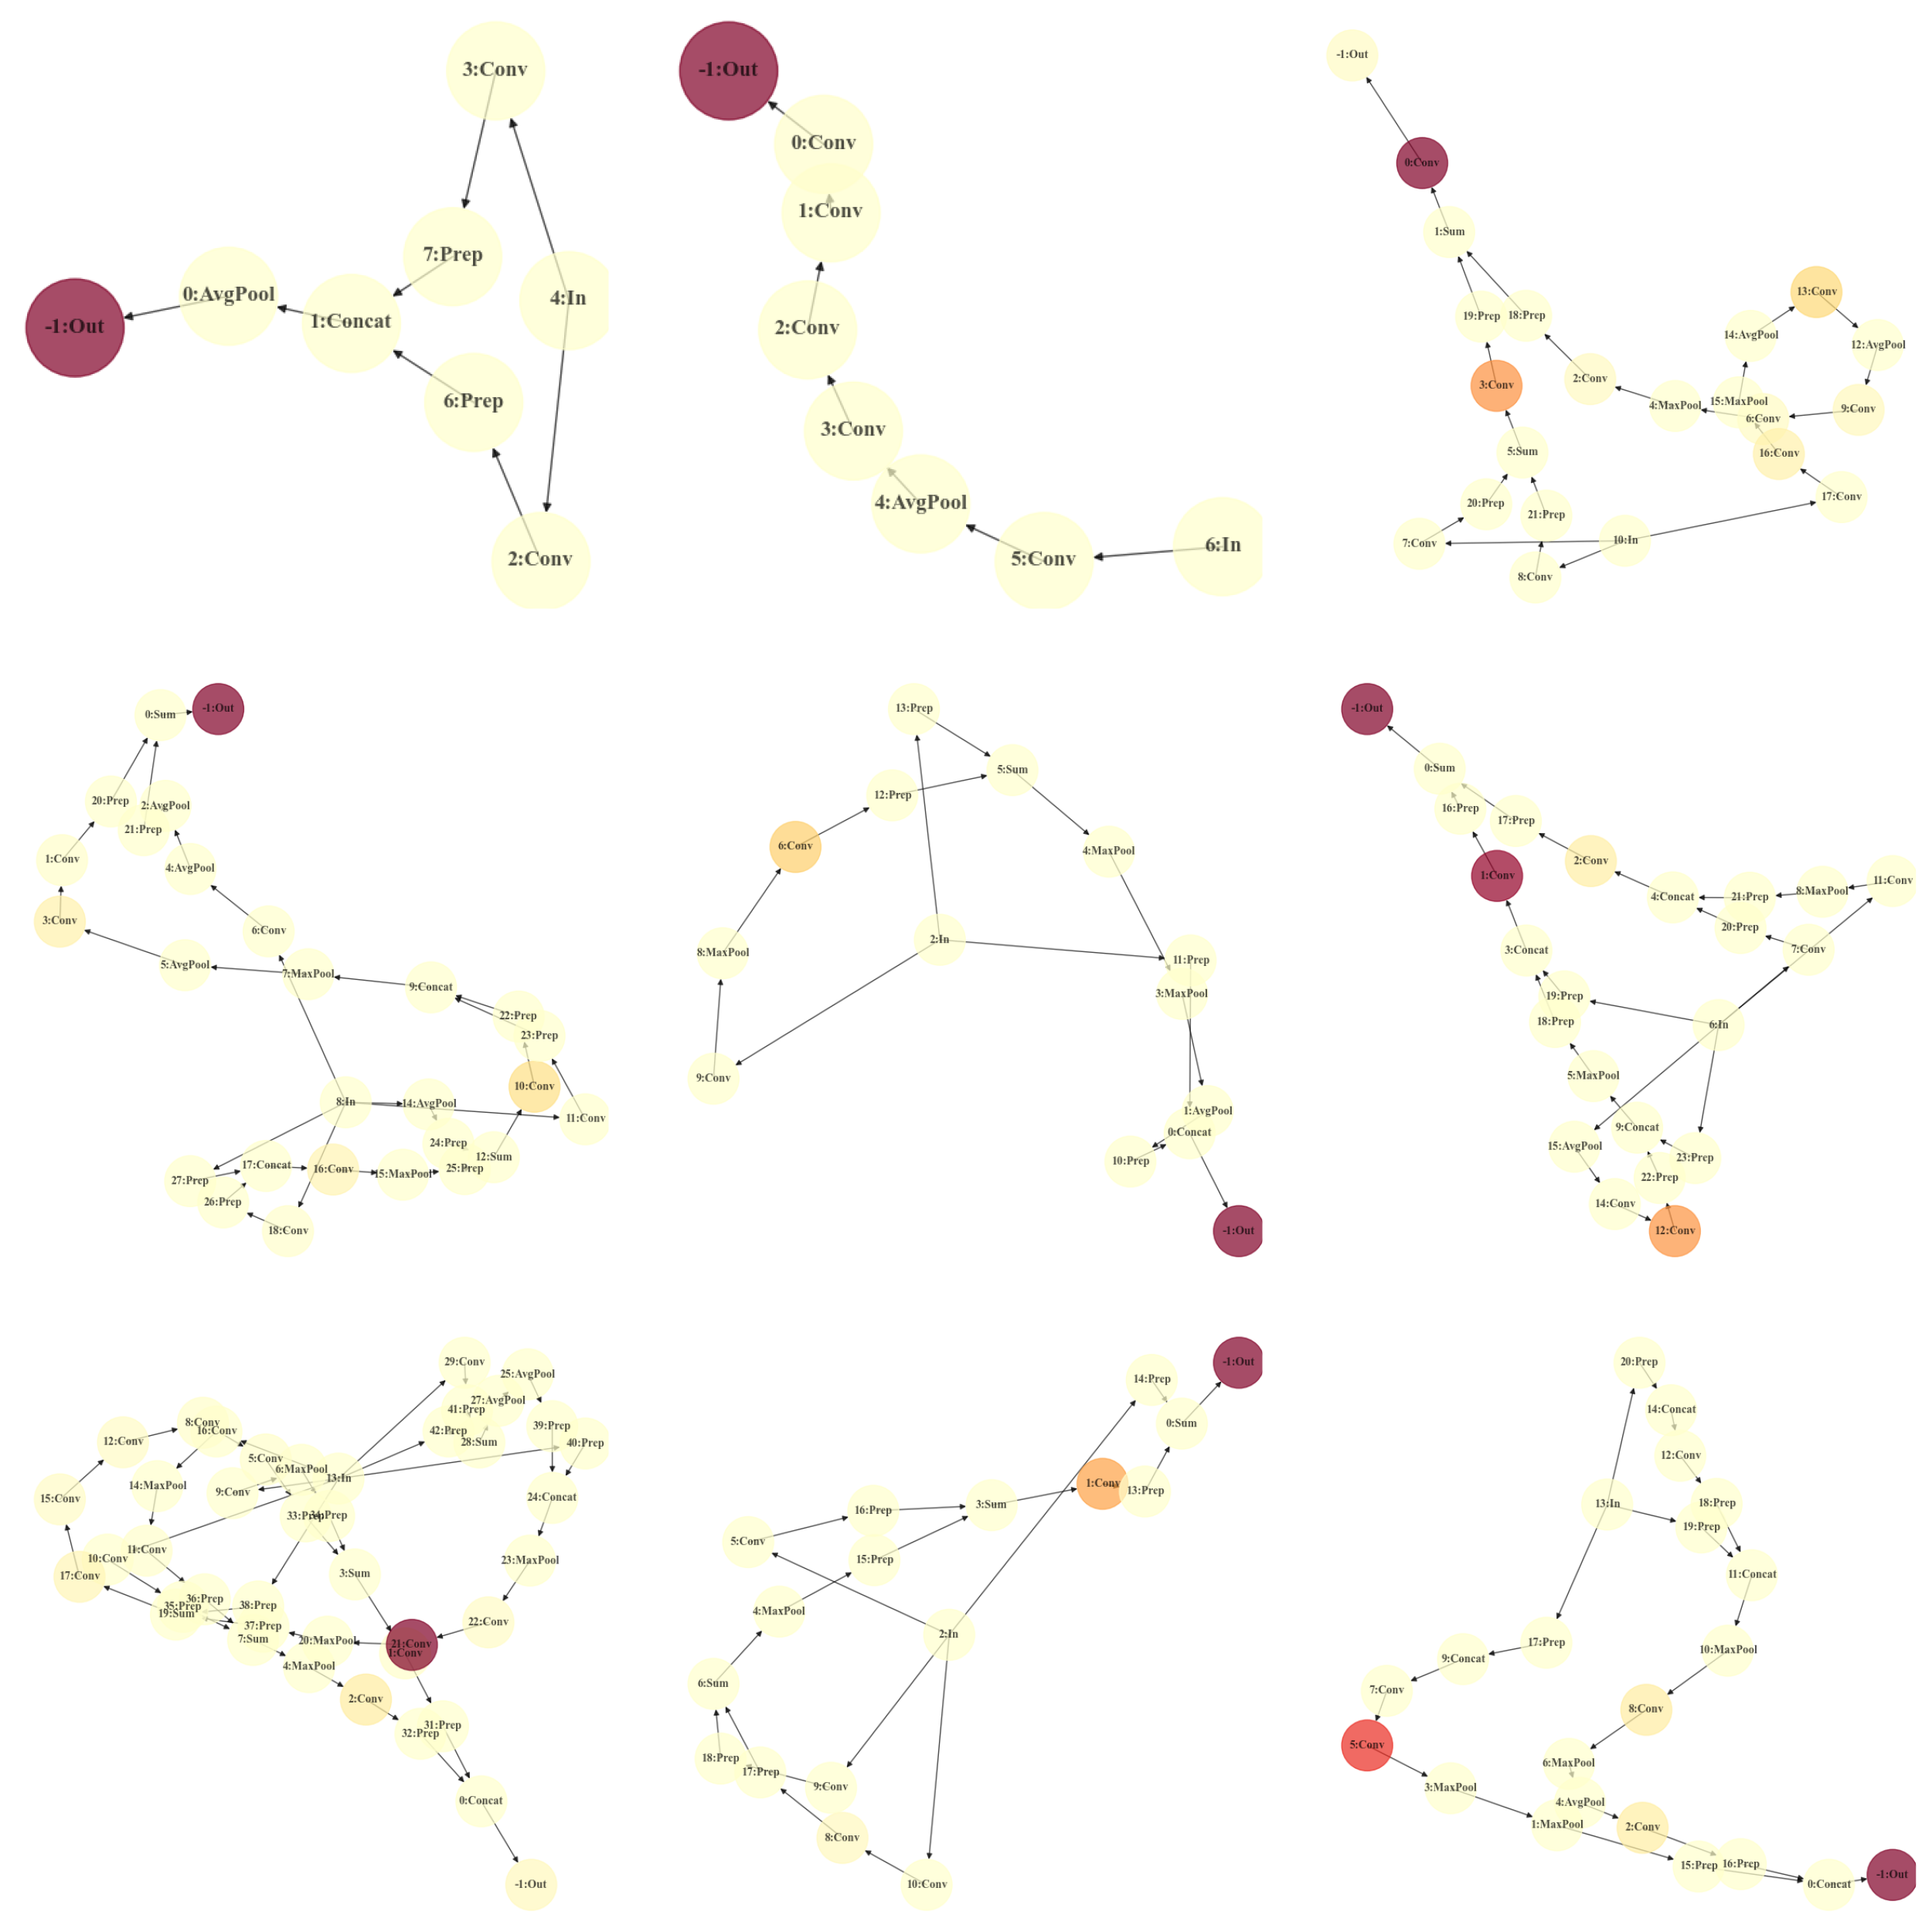
\includegraphics[width=0.8\textwidth]{4_results/imgs/ras/grid.png}
            \caption{Variety of different randomly generated neural architectures. Lighter: None or few parameters, Darker: significant percentage of all parameters.}
        \end{figure}

\newpage
        \subsection{Performance}

The algorithm was tested against two different datasets to assess whether the method has any real world applicability. The two test datasets are; the MNIST hand writen digit recognition dataset, and the CIFAR\_10 dataset which is a large corpus of small $32 \times 32$  images comprising 10 different categories.

The MNIST dataset was trained in batches of 8 images for 800 iterations and 1 epoch. The CIFAR\_10 dataset was trained in batches of 8 images for 1000 iterations and 1 epoch. The aim was to:

\begin{enumerate}
    \item test if the algorithm could produce networks capable of learning the tasks at hand;
    \item assess the learning speed of varying models
\end{enumerate}

The results for each experiment are show below.

            \subsubsection{MNIST}
            The MNIST dataset proved rather trivial to learn. Models were generated that could achieve 95\% accuracy in such a limited amount of training.
                \begin{figure}[h]
                        \centering
                        \label{fig:mnist_train}
                        \includegraphics[width=0.9\textwidth]{4_results/imgs/mnist/Training_loss}
                    \caption{Training performance on MNIST for a generation of networks. Loss is categorical cross entropy.}
                \end{figure}


                \begin{figure}[h]
                        \centering
                        \label{fig:mnist_test}
                        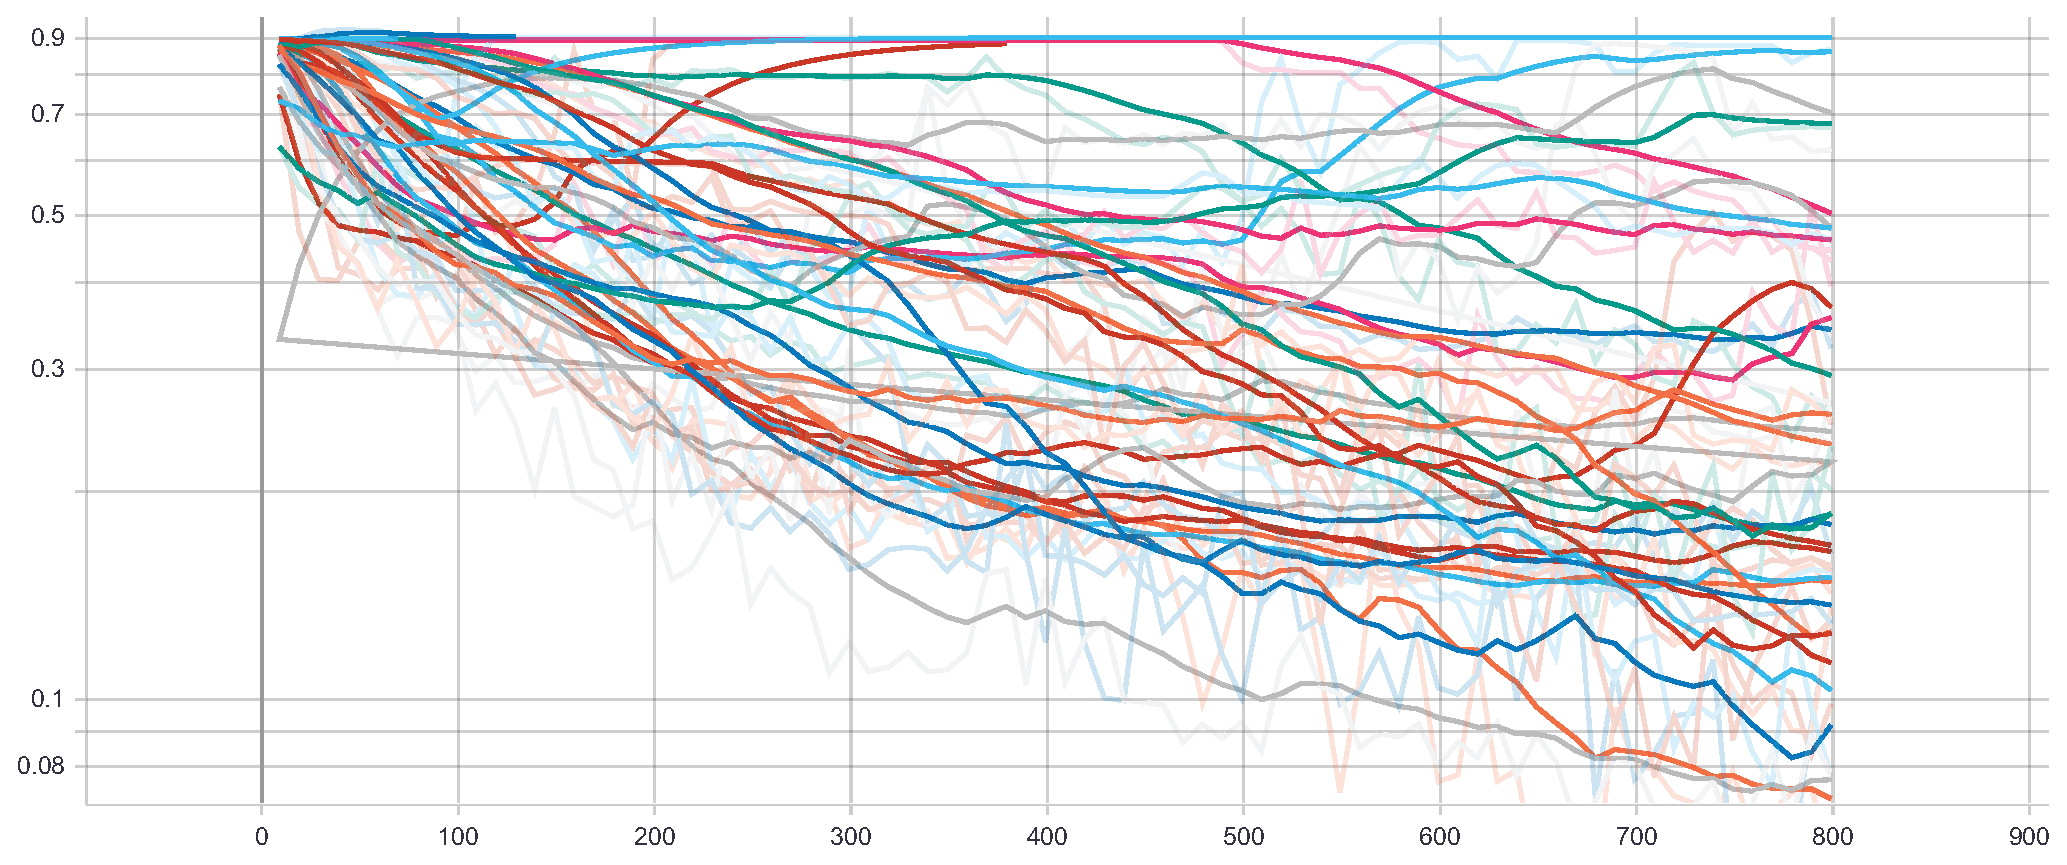
\includegraphics[width=0.9\textwidth]{4_results/imgs/mnist/Test_loss}
                    \caption{Test performance on MNIST for a generation of networks. Loss is the negative log likelihood.}
                \end{figure}


                \begin{figure}[h]
                        \centering
                        \label{fig:mnist_batch}
                        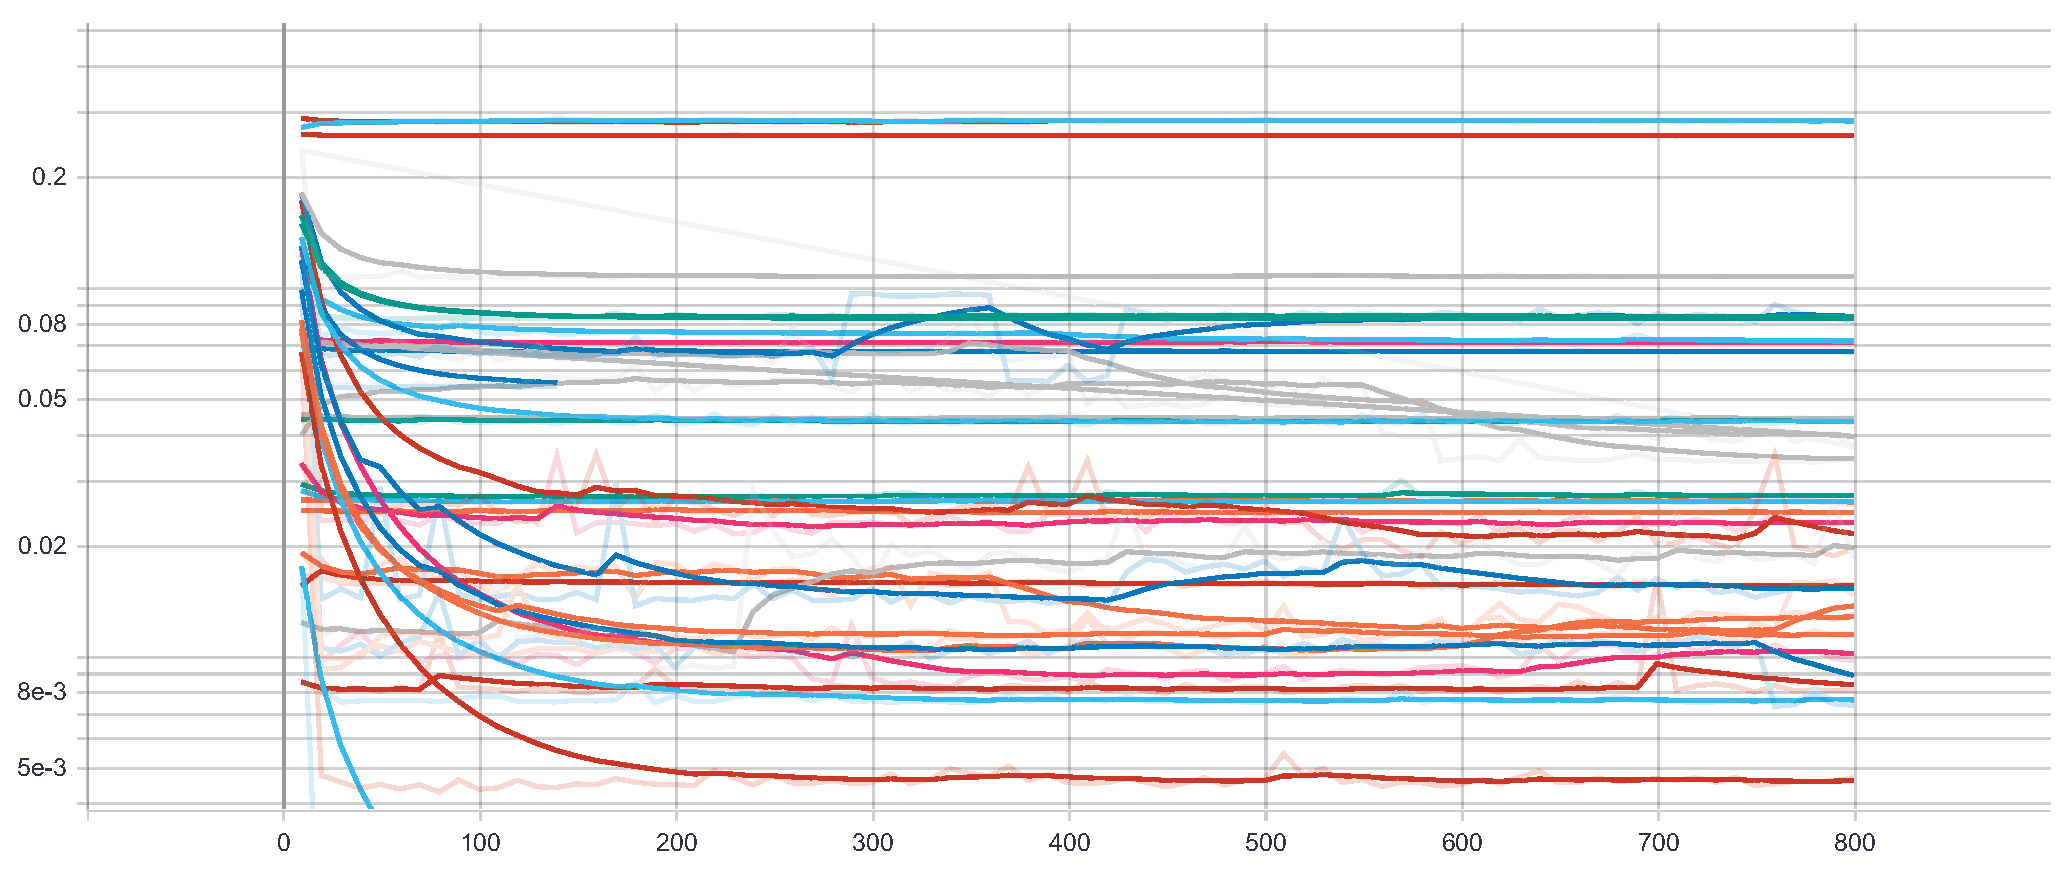
\includegraphics[width=0.9\textwidth]{4_results/imgs/mnist/Average_batch_time}
                    \caption{Average batch processing time over training steps on MNIST.}
                \end{figure}


                \begin{figure}[H]
                        \centering
                        \label{fig:mnist_predit}
                        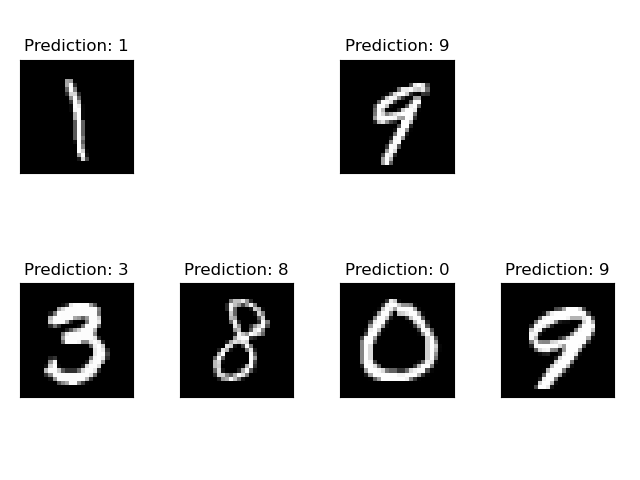
\includegraphics[width=0.6\textwidth]{4_results/imgs/mnist/predict}
                    \caption{Prediction of best model.}
                \end{figure}


\clearpage
\pagebreak
\newpage

        \subsubsection{CIFAR10}
        The CIFAR\_10 dataset proved to be far more difficult to learn with such limited training time.
        This is is part of the motivation for including this dataset, to truly test its ability. No model could achieve better than 40\% accuracy in this task, and training times were long as opposed to the MNIST dataset. The networks were allowed to grow larger than that in the MNIST experiment owing to the greater complexity of the data. As such, the accuracy divided by the $\log(parameters)$ was recorded to try to gain an understanding of how the number of parameters affected model performance during training. Figure \ref{fig:cifar_10_predit} illustrates the poor performance of even the best model.
                \begin{figure}[h]
                        \centering
                        \label{fig:cifar_10_train}
                        \includegraphics[width=0.9\textwidth]{4_results/imgs/cifar_10/Training_loss}
                    \caption{Training performance on CIFAR\_10 for a generation of networks. Loss is categorical cross entropy.}
                \end{figure}


                \begin{figure}[h]
                        \centering
                        \label{fig:cifar_10_test}
                        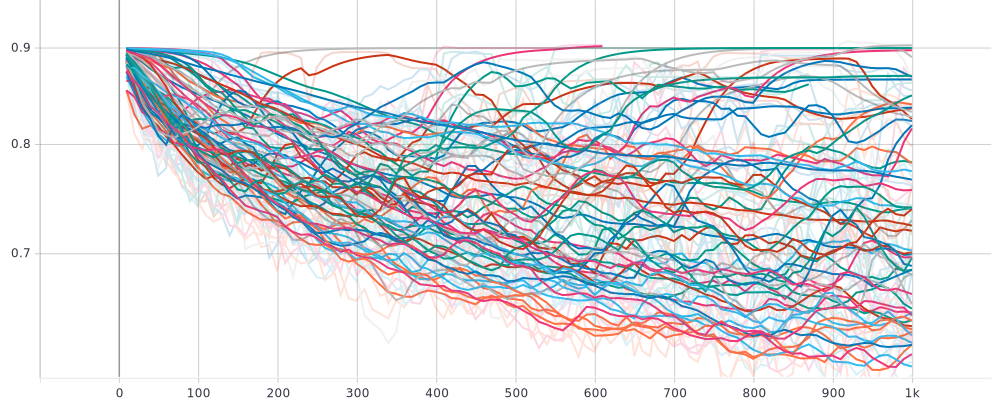
\includegraphics[width=0.9\textwidth]{4_results/imgs/cifar_10/Test_loss}
                    \caption{Test performance on CIFAR\_10 for a generation of networks. Loss is the negative log likelihood.}
                \end{figure}

                \begin{figure}[h]
                        \centering
                        \label{fig:cifar_10_accuracy}
                        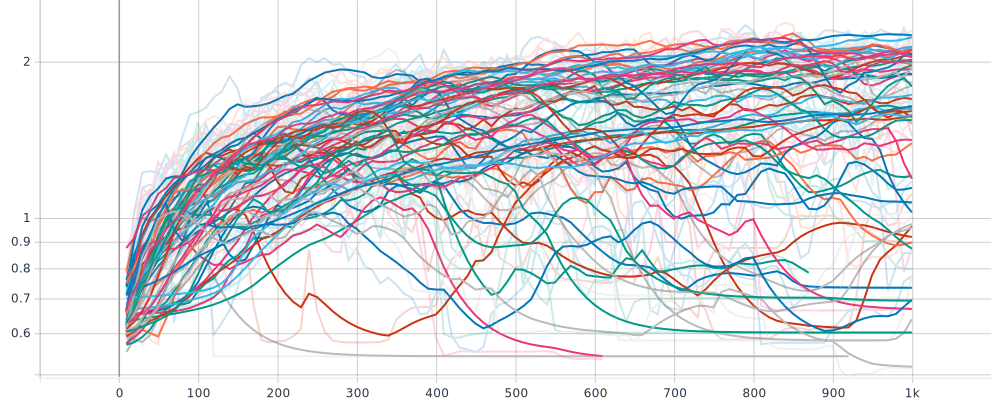
\includegraphics[width=0.9\textwidth]{4_results/imgs/cifar_10/Accuracy_vs_log(parameters)}
                    \caption{Accuracy divided by $\log(paramaters)$ over training steps for CIFAR\_10}
                \end{figure}

                \begin{figure}[h]
                        \centering
                        \label{fig:cifar_10_batch}
                        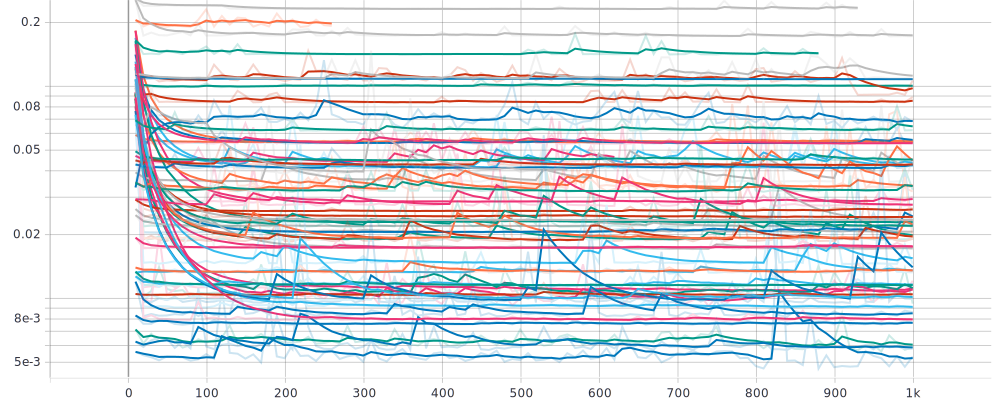
\includegraphics[width=0.9\textwidth]{4_results/imgs/cifar_10/Average_batch_time}
                    \caption{Average batch processing time over training steps on CIFAR\_10.}
                \end{figure}

                \begin{figure}[h]
                        \centering
                        \label{fig:cifar_10_predit}
                        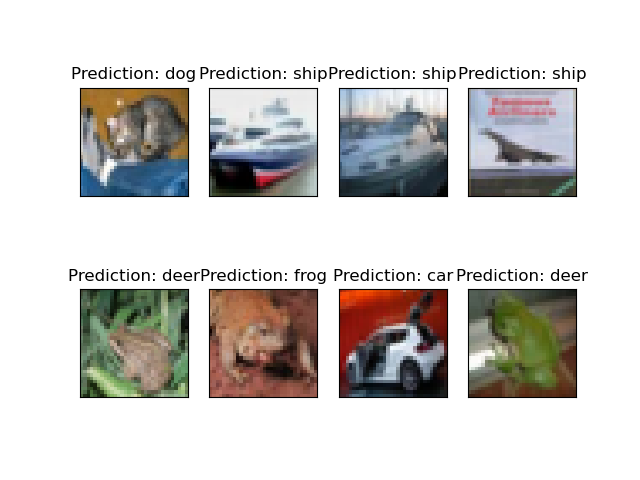
\includegraphics[width=0.7\textwidth]{4_results/imgs/cifar_10/predict}
                    \caption{Prediction of best model.}
                \end{figure}
